\documentclass[a4paper]{article}
\usepackage[utf8]{inputenc}
\usepackage[spanish, es-tabla]{babel}

\usepackage{amsmath}
\usepackage{amsfonts}
\usepackage{amssymb}
\usepackage{float}
\usepackage{graphicx}

\graphicspath{ {./Imagenes/} }

\usepackage{multirow}
\setlength{\doublerulesep}{\arrayrulewidth}

\usepackage{array}
\newcolumntype{C}[1]{>{\centering\let\newline\\\arraybackslash\hspace{0pt}}m{#1}}

\usepackage[american]{circuitikz}

\usepackage{fancyhdr}

\usepackage{units} 

\pagestyle{fancy}
\fancyhf{}
\lhead{22.42 Laboratorio de Electrónica}
%\rhead{Bertachini, Lambertucci, Londero, Mechoulam}
\rfoot{Página \thepage}


\begin{document}

%%%%%%%%%%%%%%%%%%%%%%%%%%%%%%%%%%%%%%%%%%%%%%%%%%%%%%%%%%%%%%%%%%%%%%%%% 
%								CARATULA								%
%%%%%%%%%%%%%%%%%%%%%%%%%%%%%%%%%%%%%%%%%%%%%%%%%%%%%%%%%%%%%%%%%%%%%%%%% 

\begin{titlepage}

\newcommand{\HRule}{\rule{\linewidth}{0.5mm}}
\center
\mbox{\textsc{\large \bfseries {INSTITUTO TECNOLÓGICO DE BUENOS AIRES}}}\\[1cm]
\textsc{\Large 22.42 Laboratorio de Electrónica}\\[0.5cm]


\HRule \\[0.6cm]
{ \Huge \bfseries Trabajo Práctico N$^{\circ}$4}\\[0.4cm] 
\HRule \\[1.5cm]


{\large

\emph{Grupo 3}\\
\vspace{3px}

\begin{tabular}{lr} 	
\textsc{Bertachini}, Germán  & 58750 \\ 	
\textsc{Lambertucci}, Guido Enrique  & 58009 \\
\textsc{Londero Bonaparte}, Tomás Guillermo  & 58150 \\
\textsc{Mechoulam}, Alan  &  58438\\
\textsc{Scapolla}, Franco & 58465
\end{tabular}

\vspace{20px}

\emph{Profesores}\\
\vspace{3px}
\textsc{Cossutta}, Pablo Martín\\
\textsc{Weill}, María\\
\textsc{Salvati}, Matías\\	
\vspace{100px}

\begin{tabular}{ll}

Presentado: & 15/10/19\\

\end{tabular}

}

\vfill

\end{titlepage}



%%%%%%%%%%%%%%%%%%%%%%%%%%%%%%%%%%%%%%%%%%%%%%%%%%%%%%%%%%%%%%%%%%%%%%%%% 
%								INFORME									%
%%%%%%%%%%%%%%%%%%%%%%%%%%%%%%%%%%%%%%%%%%%%%%%%%%%%%%%%%%%%%%%%%%%%%%%%%


%%%%%%%%%%%%%%%%%%%%%%%%%%%%%%%%%%%%%%%%%%%%%%%%%%%%%%%%%%%%%%%%%%%%%%%%% 
%					RECORTAR IMAGEN DEL OSCILOSCOPIO					%
%%%%%%%%%%%%%%%%%%%%%%%%%%%%%%%%%%%%%%%%%%%%%%%%%%%%%%%%%%%%%%%%%%%%%%%%%

%\begin{figure}[H]
%	\centering
%	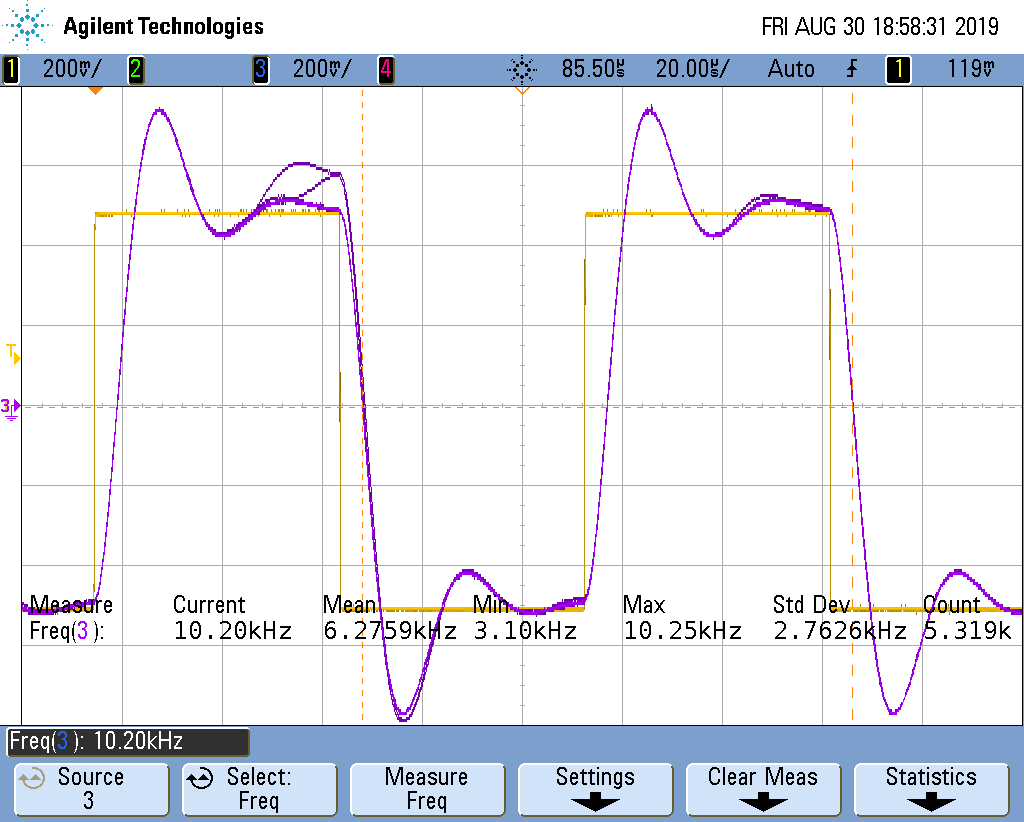
\includegraphics[width=0.9\textwidth , trim={0.7cm 6.25cm  0 3.5cm},clip]{scope_1}
%	%trim={<left> <lower> <right> <upper>}
%\caption{...}
%	\label{fig:...}
%\end{figure}



\section*{Introducción}

En el siguiente informe se realizan diversas mediciones con el osciloscopio, con el objetivo de mejorar el manejo y comprensión de dicho instrumento.

\section*{Desarrollo de la Experiencia}

\subsection*{Filtro Pasa-bajos de Primer Orden}

Se realiza en un protoboard el circuito mostrado en la figura (\ref{figure:circuito_Pasa-bajos}). Para esto se utilizó una resistencia $ R = 3,9 \ k\Omega $ y un capacitor $ C = 2,2 \ nF $. Ademas, se utilizó el analizador de impedancia con ambos componentes para medir sus valores reales obteniendose los valores expresados en la tabla (\ref{table:valores_calculados}):


%Circuito pasabajo

	\begin{figure}[h!]
	\centering
  \begin{circuitikz}[scale=1.6]\draw
	(0,2) to[V, l=$V_{inp}$,a=$10 V_{pp}$,*-*] (0,0)
	(0,2) to[R, i=i(t), v=$V_r$,l=$R$,,*-*] (4,2)
	(4,2) to[C, v=$V_c$,l=$C$, *-*] (4,0)
	(0,0) -- (4,0)

	(2,0) node[ground] {}
	(2,0) node[circ]{}
	(0,2) node[circ]{}

 	{[anchor=south east]  (0,2) node {A} (4,2) node {B} (4,0) node {C} };
 	\end{circuitikz}

 \caption{Filtro pasabajos}
\label{figure:circuito_Pasa-bajos} 
   \end{figure}
 
 %~Circuito pasabajo
 


Con la fuente, se aplicó una tensión senoidal de una amplitud de $9,78 \ V$ para determinar la frecuencia de resonancia real de dicho circuito, obteniéndose así una frecuencia de $18,5 \ k\ Hz$. Luego, midiéndose la tensión del capacitor, se busca calcular el valor de capacitancia y de esta forma calcular el error existente entre el valor de calculado de esta forma y el obtenido por el analizador de impedancia. Utilizando el valor teórico de la resistencia se obtiene lo siguiente:
%% Valores obtenidos
 \begin{center}
     \begin{table}[H]
     \centering

     \label{table:valores_calculados}
         \begin{tabular}{|c|c|c|c|}
            \hline 
              R &  $C_{calculado}$ &    $C_{medido}$   &  Error\\
            \hline 
            $R_T = 3k90\Omega$  & $2.2126nF$ & $2.2297nF$ & $1.13\%$ \\ \hline  
            $R_M = 3k87\Omega$ & $2.2297nF$ & $2.2297nF$ & $0.37 \%$ \\   \hline
        \end{tabular}
        \caption{Valores obtenidos}
    \end{table}
\end{center}
%% ~Valores obtenidos

Se retira el capacitor y se repiten las mediciones realizadas con el objetivo de calcular la capacidad de las puntas del osciloscopio. De esta forma se obtiene un error de $ ???  $ con el valor teórico de la resistencia, y un error de $  ???  $ con el medido.
A continuación, se mide la diferencia de fase entre la corriente y la tensión en el capacitor, y se verifica la suma vectorial de las tensiones, es decir $ \overrightarrow{V} = \overrightarrow{V_R} \ + \ \overrightarrow{V_C} $.



Posteriormente se calcula analíticamente la transferencia del circuito, llegándose a la expresión

\begin{equation}
	H \left(S \right) = \frac{V_C}{V} = \frac{1}{SCR + 1} = \frac{1}{S \cdot 8.58 \cdot 10^{-6} + 1}
	\label{equ:transfpasabajos}
\end{equation}

Ademas, partiendo de una frecuencia de $ 10 \ Hz $ hasta llegar a $ 1 \ MHz $, se toman varios valores tanto de la tensión del capacitor como de la fuente. De esta forma, se grafica punto a punto la transferencia y se la compara con la teórica hallada en (\ref{equ:transfpasabajos}).

%\begin{figure}[H]
%	\centering
%	\includegraphics[width=0.9\textwidth]{}
%	\caption{Transferencia teórica y medida del circuito \ref{graf:pasabajos}.} 
%	\label{graf:transfpasabajos}
%\end{figure}

Luego, se mide la tensión de la resistencia ...

%% Valores obtenidos Bode pasabajos
 \begin{center}
     \begin{table}[H]
     \centering
     \renewcommand{\arraystretch}{1.1}
     \label{table:Filtro pasabajos}
         \begin{tabular}{ c c c c c c c c }
            \hline 
             Medici\'on &  $|V|$ & $|V_c|$& $|V_R|$ & f & $\frac{V_c}{V}[dB]$ & $\theta_{\Delta t}$  &  $\theta_{XY}$\\
             \hline
                1&	9.94&	9.94&	0.00&	10&		0.00& &\\
				2&	9.81&	9.81&	0.00&	500&	0.00& &\\
				3&	9.81&	9.77&	0.04&	1000&	0.04& &\\
				4&	9.81&	9.68&	0.13&	1200&	0.12& &\\
				5&	9.81&	9.62&	0.19&	1800&	0.17& &\\
				6&	9.81&	9.58&	0.23&	3000&	0.21& &\\
				7&	9.81&	9.44&	0.37&	5000&	0.33& &\\
				8&	9.81&	9.06&	0.75&	8000&	0.69& &\\
				9&	9.81&	8.61&	1.20&	10000&	1.13& &\\
				10&	9.81&	7.94&	1.87&	14000&	1.84& &\\
				11&	9.81&	7.38&	2.43&	16000&	2.47& &\\
				12&	9.81&	6.81&	3.00&	18000&	3.17& &\\
				13&	9.81&	6.70&	3.11&	20000&	3.31& &\\
				14&	9.81&	6.44&	3.37&	22000&	3.66& &\\
				15&	9.81&	5.31&	4.50&	30000&	5.33& &\\
				16&	9.81&	3.56&	6.25&	50000&	8.80& &\\
				17&	9.81&	2.38&	7.43&	80000&	12.30& &\\
				18&	9.81&	1.69&	8.12&	120000&	15.28& &\\
				19&	9.81&	1.44&	8.37&	150000&	16.67& &\\
				20&	9.81&	1.19&	8.62&	180000&	18.32& &\\
				21&	9.81&	1.13&	8.68&	200000&	18.77& &\\
				22&	9.81&	0.44&	9.37&	250000&	26.96& &\\
				23&	9.81&	0.81&	9.01&	300000&	21.66& &\\
				24&	9.81&	0.56&	9.25&	500000&	24.87& &\\
				25&	9.81&	0.30&	9.51&	1000000&	30.29& &\\

            \hline 
        \end{tabular}
        \caption{H(\$) - Filtro pasabajos}
    \end{table}
\end{center}
%%~Valores obtenidos Bode pasabajos

\subsection*{Filtro Pasa-altos de Primer Orden}

Con los mismos elementos utilizados para armar el circuito (\ref{graf:pasabajos}), se elabora el circuito pasaaltos de la figura (\ref{graf:pasaaltos}). Su transferencia se calcula analíticamente obteniéndose:

\begin{equation}
	H \left(S \right) = \frac{V_C}{V} = \frac{SCR}{SCR + 1} = \frac{S \cdot 8.58 \cdot 10^{-6}}{S \cdot 8.58 \cdot 10^{-6} + 1}
	\label{equ:transfpasaaltos}
\end{equation}

%Circuito pasaalto
  \begin{center}\begin{circuitikz}[scale=1.6]\draw
(0,2) to[V, l=$V_inp$,a=$10 V_{pp}$,*-*] (0,0)
(0,2) to[C, v=$V_c$,l=$C$, *-*] (4,2)
(4,2) to[R, i=i(t), v=$V_r$,l=$R$,,*-*] (4,0)
(0,0) -- (4,0)

(2,0) node[ground] {}
(2,0) node[circ]{}
(0,2) node[circ]{}

 {[anchor=south east]  (0,2) node {A} (4,2) node {B} (4,0) node {C} };\end{circuitikz} \end{center}
 %~Circuito pasaalto

Al igual que con el filtro pasabajos, se procede a medir varios puntos de la tensión de la resistencia y de la fuente, variando la frecuencia. Así se grafica la transferencia medida y se la compara con la teórica hallada en (\ref{equ:transfpasaaltos}).

%% Valores obtenidos Bode pasaltos
 \begin{center}
     \begin{table}[H]
     \centering
	   \renewcommand{\arraystretch}{1.1}
     \label{table:Filtro pasaalto}
         \begin{tabular}{c c c c c c }
            \hline 
             Medici\'on  & $|V_{in}|$ &    $|V_r|$ & f&  $\frac{V_r}{V}[dB]$ & $\theta_{\Delta t}$  \\
             \hline
                1	&9.94&	0.075	&10	    &42.45 & \\
                2	&9.94&	0.6	    &500	&24.38 & \\
                3	&9.94&	0.9	    &1000	&20.86 & \\
                4	&9.94&	1.1	    &1200	&19.12 & \\
                5	&9.94&	1.3 	&1800	&17.67 & \\
                6	&9.94&	2	    &3000	&13.93\\
                7	&9.94&	3.11	&5000	&10.09\\
                8	&9.94&	4.41	&8000	&7.06\\
                9	&9.94&	4.81	&10000	&6.30\\
                10	&9.94&	6.2	    &14000	&4.10\\
                11	&9.94&	6.84	&16000	&3.25\\
                12	&9.94&	6.91	&18000	&3.16\\
                13	&9.94&	7.01	&20000	&3.03\\
                14	&9.94&	7.28	&22000	&2.71\\
                15	&9.94&	8.23	&30000	&1.64\\
                16	&9.94&	8.93	&50000	&0.93\\
                17	&9.94&	9.31	&80000	&0.57\\
                18	&9.94&	9.69	&120000	&0.22\\

 \hline
        \end{tabular}
        \caption{H(\$) - Filtro pasaalto}
    \end{table}
\end{center}

%% ~Valores obtenidos Bode pasaaltos

A continuación, se reemplaza la tensión sinusoidal por una triangular, variando la frecuencia. ...

\textbf{Mostrar 3 gráficos representativos y sacar conclusiones. En el caso mas apropiado medir la respuesta transitoria y en caso de ser viable, demostrar analíticamente lo obtenido}

\subsection*{Sincronización de Instrumentos}
En este punto se utiliza el barrido automático del generador de funciones, para visualizar en el osciloscopio la respuesta en frecuencia del circuito de la la figura (\ref{graf:pasabajos}). Se realizó la medición aproximada utilizando dos métodos.

\subsubsection*{Modo XY con dos Generadores}
Este método consiste en utilizar un generador para realizar el barrido por el eje horizontal del osciloscopio mientras que se usa otro para barrer a lo largo de las frecuencias en el circuito, que se mostrará en el eje Y.

\begin{figure}[H]
	\centering
	%\includegraphics[width=0.8\textwidth,trim={0.5cm 2cm  0.5 5cm},clip]{oscixxx.png}
	\caption{Medición de la respuesta en frecuencia del circuito de la figura \ref{graf:pasabajos} utilizando el método XY y dos generadores.} 
	\label{graf:osci_freq_alta}
\end{figure}

\subsubsection*{Modo Normal}
Por otro lado, se utilizó el modo normal, disparado acordemente, es decir, utilizando un solo generador de funciones.
\begin{figure}[H]
	\centering
%	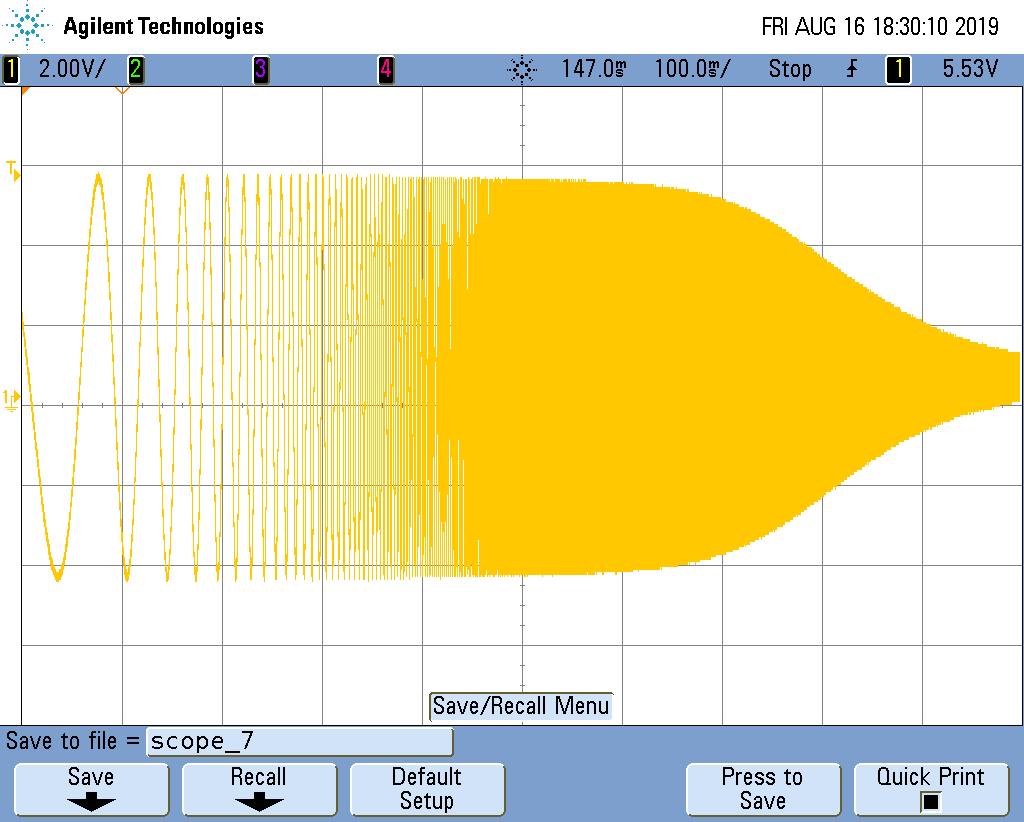
\includegraphics[width=0.8\textwidth,trim={0.5cm 2cm  0.5 5cm},clip]{ej3normal.png}
	\caption{Medición de la respuesta en frecuencia del circuito de la figura \ref{graf:pasabajos} utilizando el modo normal del trigger.} 
	\label{graf:ej3modonormal}
\end{figure}
Se utilizó un barrido en frecuencia desde $100 \ mHz$ hasta $70 \ kHz$, en un período total de 2 segundos con una amplitud de 5 volt pico a pico. Para lograr visualizar la mayor parte de la respuesta en frecuencia, se utilizó el modo Single del osciloscopio, con el trigger en una amplitud igual a la de la salida al comienzo del barrido. Se observa que este modo de usar el osciloscopio puede ser una forma fácil de visualizar a la respuesta en frecuencia de un circuito de forma rápida y muy aproximada.

\subsection*{Respuesta en Frecuencia del Osciloscopio}
Finalmente, se midió la respuesta en frecuencia del Agilent DSO6014A del laboratorio, activando los filtros AC y BW. Se esperaba, según la teoría, que la respuesta sea similar a la de un filtro pasa-banda, atenuando las frecuencias muy bajas y muy altas. Esto es, realizando a priori la suposición de que el generador de funciones nos proporcionará una amplitud de señal constante a todas las frecuencias.

Para realizar la medición, se conectó el osciloscopio con las puntas en x10 previamente calibradas, se activaron los filtros y se conectaron las puntas del osciloscopio a la salida de un generador de funciones con una señal sinusoidal de amplitud pico a pico de 20 voltios para minimizar la lectura de ruido. Se comenzó a medir desde una frecuencia muy pequeña, de $10 \ mHz$, como se puede ver en la figura \ref{graf:osci_freq_baja}. Se finalizó la medición con la mayor frecuencia que admite el generador usado, de $15 \ MHz$, observado en la figura \ref{graf:osci_freq_alta}.

\begin{figure}[H]
	\centering
%	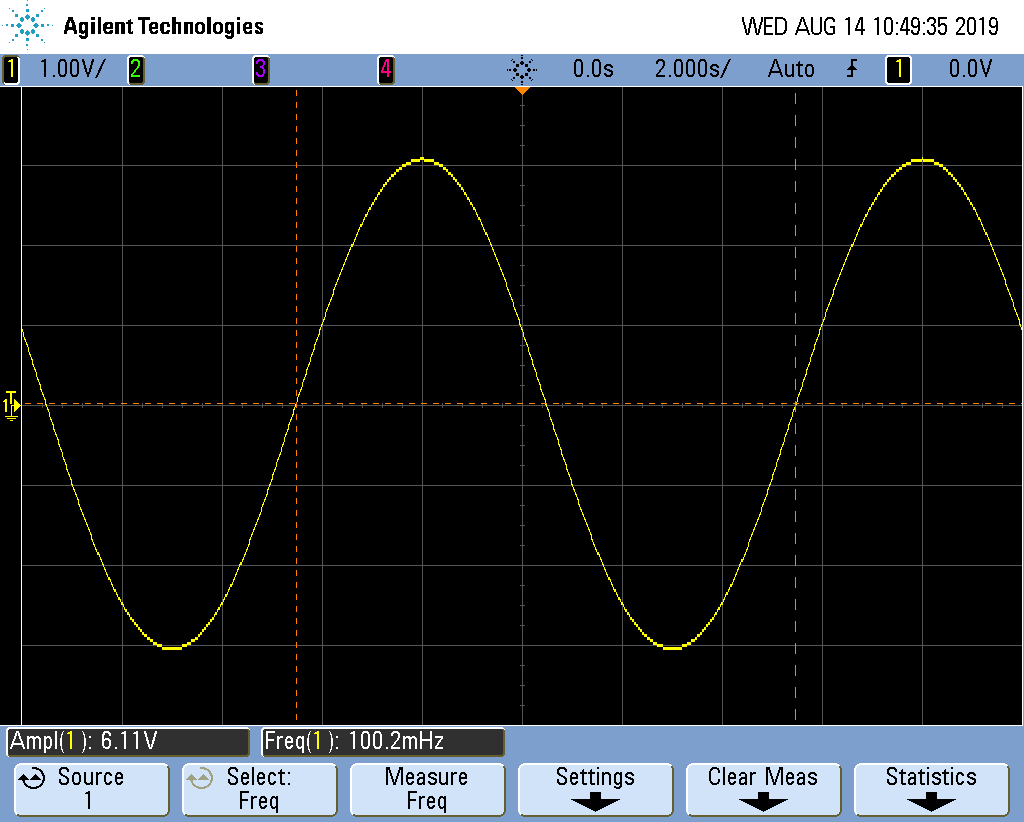
\includegraphics[width=0.8\textwidth,trim={0.5cm 2cm  0.5 5cm},clip]{osci100mhz.png}
	\caption{Medición de la respuesta en frecuencia del osciloscopio a una frecuencia de $1 \ Hz$ con los filtros BW y AC. (500ms/div)} 
	\label{graf:osci_freq_baja}
\end{figure}

\begin{figure}[H]
	\centering
%	\includegraphics[width=0.8\textwidth,trim={0.5cm 2cm  0.5 5cm},clip]{osci15Mhz.png}
	\caption{Medición de la respuesta en frecuencia del osciloscopio a una frecuencia de $15 \ MHz$ con los filtros BW y AC.} 
	\label{graf:osci_freq_alta}
\end{figure}


Finalmente, se utilizó python para graficar la respuesta en frecuencia en amplitud del osciloscopio con los filtros BW y AC, observado en la figura \ref{graf:resp_freq_osci}.

\begin{figure}[H]
	\centering
%	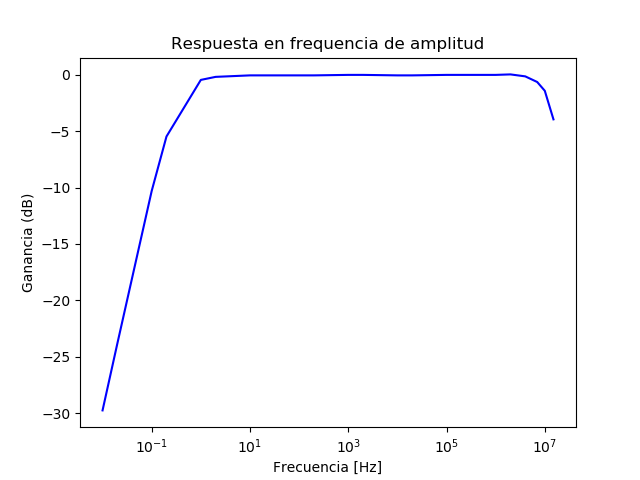
\includegraphics[width=0.8\textwidth]{resp_freq_osci.png}
	\caption{Gráfico de la respuesta en frecuencia del DSO6014A con los filtros BW y AC.} 
	\label{graf:resp_freq_osci}
\end{figure}

Se puede observar que en la práctica la respuesta en frecuencia del osciloscopio resulta ser un pasabanda, que atenua frecuencias menores a $\approx 5 \ Hz$ y mayores a $\approx 1 \ MHz$. Estos resultados verifican la suposición hecha con ayuda de los conocimientos de la teoría. Se observa también que los filtros utilizados limitan al osciloscopio en ancho de banda significantemente, ya que según el fabricante la frecuencia a la que se atenúan las señales por $3dB$ es de $100 \ MHz$, mientras que en la figura \ref{graf:resp_freq_osci} puede verse que esa frecuencia es de $\approx 10-15 \ MHz$. Además, se puede notar como a $\approx 15 \ MHz$ se comienza a deformar la señal sinusoidal significantemente.\\

Si se comparan los datos obtenidos con los datos del fabricante:
\begin{center}
BANDWIDTH $\rightarrow$ MSO/DSO601xA: DC to 100 MHz\\
AC-COUPLED $\rightarrow$ MSO/DSO601xA: 3.5 Hz to 100 MHz\\
BW LIMIT $\rightarrow$ MSO/DSO601xA: 20 MHz selectable\\
\end{center}
se puede ver que la práctica concuerda aproximadamente con los datos provistos.

\end{document}
